%Sagarmatha Engineering College Project Report Template
\documentclass[12pt,a4paper,oneside]{report}
\usepackage[titles]{tocloft}

\usepackage{multirow}
\usepackage{rotating}
\usepackage{hhline}
\usepackage{graphicx}
\graphicspath{{./Graphics/}} 
\usepackage[left=1.5in, right=1in,top=1in,bottom=1in,headheight=6pt, a4paper]{geometry}
\usepackage{titling}
\usepackage{booktabs}
\usepackage{natbib}
\usepackage{times}
% \usepackage{microtype}
\usepackage{amsmath}
\usepackage{enumitem}
\usepackage[font=normalsize,labelfont=bf,tableposition=top]{caption}
\usepackage{setspace}
\usepackage{tabto}
\usepackage[explicit]{titlesec}
\usepackage[absolute]{textpos}
\usepackage[export]{adjustbox}
\usepackage[T1]{fontenc}
\usepackage{float}
\usepackage{datetime}
\usepackage{fancyhdr}
\pagestyle{fancy}
\fancyhf{}
\fancyfoot[C]{\thepage}
\newdateformat{monthyeardate}{%
  \monthname[\THEMONTH], \THEYEAR}


\linespread{1.5}
\setlength{\parskip}{6pt}
\setlength{\parindent}{0em}
\titleformat{\chapter}[display]
    {\centering\normalfont\normalsize\bfseries}{\MakeUppercase{\chaptertitlename} \thechapter}{0pt}{\normalsize #1}
\titlespacing{\chapter}{0pt}{0pt}{20pt}


\titleformat{\section}
  {\normalfont\normalsize\bfseries}{\thesection}{1em}{#1}

\titleformat{\subsection}
  {\normalfont\normalsize}{\thesubsection}{1em}{#1}

\titleformat{\subsubsection}
  {\normalfont\normalsize}{\thesubsection}{1em}{#1}

\renewcommand{\baselinestretch}{1.5}



\captionsetup[table]{singlelinecheck=off}
\title{HOME AUTOMATION USING SPEECH RECOGNITION}
\author{Member1, Member2, Member3}
\date


\renewcommand{\bibname}{REFERENCES}
\renewcommand\contentsname{TABLE OF CONTENTS}
\renewcommand{\listfigurename}{LIST OF FIGURES}
\renewcommand{\listtablename}{LIST OF TABLES}




\begin{document}

\begin{titlingpage} 
    \begin{normalsize}
    \begin{center}
    
\includegraphics[width=1.3in, height=1.5in]{./Graphics/logo.png}\\
    
     \textbf{TRIBHUVAN UNIVERSITY}\\
     \textbf{INSTITUTE OF ENGINEERING}\\
    
    \textbf{\MakeUppercase PASHCHIMANCHAL CAMPUS}\\
    \textbf{\MakeUppercase{Lamachaur, Pokhara}}
    \end{center}
    \vspace{1cm}
    
    \begin{center}
    \textbf{[Subject Code: EX654]}\\
    \textbf{A PROJECT REPORT}\\
    \textbf{ON}\\
    \textbf{\MakeUppercase \thetitle} \\
    \vspace{1.5 cm}
    \textbf{SUBMITTED BY:}\\
\begin{tabular}{p{5cm} l}
    \textbf{BINAYAK SHRESTHA} & [WRC077BEI012]\\
    \textbf{PRAKANDA BHANDARI} & [WRC077BEI030]\\
    \textbf{PRATHAM ADHIKARI} & [WRC077BEI032]\\
    \textbf{SANDESH BASHYAL} & [WRC077BEI036]\\
\end{tabular}\\
    \vspace{2 cm}
    \textls{\textbf{SUBMITTED TO: }}\\
    \textbf{DEPARTMENT OF ELECTRONICS AND COMPUTER ENGINEERING}\\
    %\MakeUppercase {Pashchimanchal Campus, Lamachaur-16, Pokhara}\par\\
    \vspace{1.5cm}
    \textbf{
    {\monthyeardate\today}}
    \end{center}
    \end{normalsize}
    \end{titlingpage}
    %================================================================
    \newpage
\pagenumbering{roman}
%==============================Department Acceptance==========================
\chapter*{\MakeUppercase {Tribhuwan University}\\ \MakeUppercase{Institute of Engineering}\\ \MakeUppercase{\textbf {Pashchimanchal Campus}}\\ \MakeUppercase{Department of Electronics and Computer Engineering}}
\addcontentsline{toc}{chapter}{DEPARTMENTAL ACCEPTANCE}
% \begin{tabular}{p{5.7in}}
% \noindent
\justify{
The undersigned certify that they have read, and recommended to the Institute of Engineering for acceptance, a project report entitled \textbf{"HOME AUTOMATION USING SPEECH RECOGNITION"}, submitted by Binayak Shrestha, Prakanda Bhandari, Pratham Adhikari, and Sandesh Bashyal in partial fulfilment of the requirements for the Bachelor degree in ``Electronics, Communication and Information Engineering" has been accepted as a bonafide record of work independently carried out by team in the department.\par}
% \end{tabular}

\vspace{1cm}
\line(1,0){200}\\
Supervisor: Suraj Basant Tulachan\\
Department of Electronics and Computer Engineering\\

\vspace{1cm}
\line(1,0){200}\\
External Examiner\\

\vspace{1cm}
\line(1,0){200}\\
Khemraj Koirala\\
Head of the Department\\
Department of Electronics and Computer Engineering\\
\vspace*{\fill}

\textbf {\MakeUppercase{Date of approval:} \monthyeardate\today}

%=======================================================================
\newpage
\pagenumbering{roman}
\setcounter{page}{2}
\chapter*{COPYRIGHT ©}
\addcontentsline{toc}{chapter}{COPYRIGHT}
\justify
The author has agreed that the Library, Department of Electronics and Computer
Engineering, Pashchimanchal Campus, Institute of Engineering may make this report
freely available for inspection. Moreover, the author has agreed that permission for
extensive copying of this project report for scholarly purpose may be granted by the
supervisors who supervised the project work recorded herein or, in their absence, by the
Head of the Department wherein the project report was done. It is understood that the
recognition will be given to the author of this report and to the Department of
Electronics and Computer Engineering, Pashchimanchal Campus, Institute of
Engineering in any use of the material of this project report. Copying or publication or
the other use of this report for financial gain without approval of to the Department of
Electronics and Computer Engineering, Pashchinamchal Campus, Institute of
Engineering and author’s written permission is prohibited.
Request for permission to copy or to make any other use of the material in this report in
whole or in part should be addressed to:\\
\\
Head\\
Department of Electronics and Computer Engineering\\
Pashchimanchal Campus, Institute of Engineering\\
Lamachaur, Pokhara\\
Nepal\\
\chapter*{ACKNOWLEDGEMENT}
\addcontentsline{toc}{chapter}{ACKNOWLEDGEMENT}
\justify
We would like to express our sincere gratitude to our supervisor, Mr. Suraj Basant Tulachan, for all of his help and support during the course of this project. Without a doubt, his priceless blessings and encouragement will help us move forward in life.\\
\\
Furthermore, we would like to thank the Pashchimanchal Campus, Institute of Engineering, Department of Electronics and Computer Engineering for offering us useful courses and a supportive learning environment. We sincerely appreciate all of the professors who helped and encouraged us to finish the assignment.\\
\\
Lastly, we give appreciation to the almighty, our parents, friends, and everyone who has consistently supported and encouraged us. This project would not have been possible without their help.\\


\chapter*{ABSTRACT}

\addcontentsline{toc}{chapter}{ABSTRACT}

This section consists of summary of the context

%New Paragraph
\par
\textbf{Keywords:} Deep Learning, Image colorization, EfficientNetB0, CNN, Convolution neural architecture



\renewcommand{\baselinestretch}{1.5}
\addcontentsline{toc}{chapter}{\contentsname}{\tableofcontents}
\newpage
\renewcommand\cftfigafterpnum{\baselinestretch}
\renewcommand\cftfigafterpnum{\vskip5pt\par}
\addcontentsline{toc}{chapter}{\listfigurename}{ \listoffigures}
\newpage
\addcontentsline{toc}{chapter}{\listtablename}{ \listoftables}
\newpage
\chapter*{LIST OF ABBREVIATIONS}
\addcontentsline{toc}{chapter}{LIST OF ABBREVIATIONS}
%Add abbreviations list here
AI\tabto{6em}Artificial Intelligence\\
CNN\tabto{6em} Convolution Neural Network\\
\pagenumbering{arabic}
\pagenumbering{arabic}
\setcounter{page}{1}
\chapter{INTRODUCTION}
    \section{Background}
    In the contemporary era of smart living, home automation systems have become increasingly popular due to their ability to enhance convenience, efficiency and also catering to individuals with mobility challenges. Integration of speech recognition technology into home automation systems adds an additional layer of user-friendliness, accessibility, leveraging its power to seamlessly interact with various devices within a home environment.

    Traditional method with physical switching of appliances, checking if they are on or not brings a level of inconvenience to disabled as well as abled people. This system can accurately interpret the user instructions and generates control signals for appliances. It does so by capturing audio input through a connected microphone.

    Upon receiving the audio signals, Raspberry pi utilizes a speech recognition model within it which converts the received voice data into text commands enabling the system to comprehend user instructions accurately. Once the command is interpreted, It then generates necessary control signals and sends them to a 1-channel relay module and other hardware components, allowing a seamless control of different household appliances connected to the system. The status of the appliances are updated in real-time which can be viewed on a dashboard of a web application. This system not only operates the appliances, but also views their status which makes it easier to observe them  even if  not physically present near them.

    \section{Motivation and Inspiration}
    Our project's motivation and inspiration stemmed from a genuine desire to simplify and improve daily life within homes. Witnessing the growing integration of technology into our lives, we were inspired to utilize advancements in speech recognition and automation to make household tasks more efficient and accessible. Our goal was to empower users with intuitive control over their environment, aiming for a user-friendly home automation system. Additionally, we were excited about the opportunity to explore the intersection of artificial intelligence, embedded systems, and IoT technologies, seeing it as a chance to deepen our understanding and expertise in these areas. 
    
    \section{Problem Statement}
    The absence of automated controls requires manual operation of various appliances and thus results in a time consuming routine. Managing multiple devices  manually  can be troublesome especially for elderly and the disabled. The commercial home automation systems are based mainly on Zigbee, Z-Wave, or Wi-Fi protocols. Such automated systems are either ineffective in terms of cost or power consumption. 

    Additionally, the complexity of processing speech in real-time poses a significant challenge. Existing systems often struggle with accurately interpreting the intent of the speaker. Thus, the technologies that are being applied are prone to various kinds of failures, for instance an individual’s speech can be misinterpreted,in case of multiple commands by more than one person the commands might be neglected. 

    
    \section{Objectives}
    The objectives of this project is:
        \begin{itemize}
        %define spacing
        \setlength\itemsep{1.5pt}
        %Add items
        \item To design and develop a speech recognizing home automation system that can comprehend user instructions accurately and operates accordingly.

        \end{itemize}


    \section{Scope}
    Our project's scope involves creating a comprehensive home automation system that merges speech recognition technology with hardware automation to improve household functionality. Our main goal is to develop an easy-to-use interface enabling residents to control various home fixtures and devices through voice commands. 

    We also plan to incorporate features for task scheduling, such as setting timers and activating predefined routines, to streamline daily routines further. The Raspberry Pi 4 Model B will serve as the central controlling unit, facilitating communication between the speech recognition algorithm and connected hardware components through the Arduino Nano. While our initial focus is on essential features, we're designing the system to be scalable, allowing for future expansions and updates to meet changing user needs and technological advancements in home automation.
         
\chapter{LITERATURE REVIEW}

Recurrent neural networks, long short-term memory and gated recurrent neural networks in particular, was firmly established as state of the art approaches in sequence modeling and transduction problems such as language modeling and machine translation. Numerous efforts have since continued to push the boundaries of recurrent language models and encoder-decoder architectures \cite{vaswani2017attention}.Recurrent Neural Networks (RNNs) and their variant LSTMs, while powerful, suffer from limitations. LSTMs attempt to address the vanishing gradient problem in RNNs, where crucial information from earlier parts of the sequence gets lost. However, LSTMs can still struggle with very long sequences. Additionally, both RNNs and LSTMs process information sequentially, limiting their ability to capture complex relationships within the data. This sequential nature also makes them computationally expensive for training. These drawbacks hinder their performance in tasks requiring long-range dependencies and efficient processing, paving the way for advancements like transformers.
\newline The drawbacks of these models being inability to generalize to long sequences, unparalizability are solved by Transformer.Transformers\cite{vaswani2017attention} outperform LSTMs in sequence modeling tasks like machine translation due to their powerful attention mechanism. Unlike LSTMs, which process information sequentially, transformers can attend to all parts of the input sequence simultaneously using self-attention. This allows them to capture long-range dependencies more effectively, crucial for understanding complex relationships in language. Additionally, encoders and decoders within transformers are specifically designed to handle input and output sequences, respectively, leading to better focus and efficiency compared to LSTMs' single, recurrent processing. This combination of self-attention and dedicated encoder-decoder architecture grants transformers superior accuracy in various NLP tasks. \\

For Automatic speech recognition, new speech recognition model using attention-based recurrent networks was used \cite{effectivenesschorowski2015attention}. Unlike traditional methods, the model can focus on important parts of the speech throughout the sequence. This is useful for long and noisy speech recognition tasks. The model was tested  on a phoneme recognition task and show that it performs competitively, especially for longer speech samples.\cite{effectivenesschorowski2015attention}. \newline

The Transformer model was first introduced in Gaussian mixture hidden Markov modeling for speech recognition\cite{1198704}, in order to reduce sequential calculations and the number of operations for correlating input and output position signals\cite{orken2022study}.The model performed exceptionally well in compared to state-of-the-art models at the time.

Speech recognition relies on labeled data, limiting its reach. Baevski \cite{baevski2021unsupervised} proposes wav2vec-U, an unsupervised method using self-supervised learning from wav2vec 2.0 representations. k-means clustering segments speech, and adversarial training maps segments to phonemes, even allowing for silence labels. wav2vec-U achieves significant reductions in phone error rates on TIMIT and rivals supervised models on Librispeech, demonstrating its effectiveness across languages. This approach paves the way for speech recognition in low-resource settings. Experiments on the standard Librispeech benchmark show performance close to the state of the art models from only a few years ago, even though these models relied on nearly 1,000 hours of labeled data\cite{baevski2021unsupervised}. \newline

The model, Whisper, leverages a massive dataset of audio recordings with corresponding, but imperfect, internet transcripts. This weak supervision approach, alongside multilingual and multitask training, allows Whisper to excel in zero-shot generalization and achieve competitive performance compared to fully supervised models. Furthermore, Whisper simplifies the recognition pipeline by eliminating the text normalization step. These findings highlight the potential of weak supervision for robust and efficient speech recognition.The smallest zero-shot Whisper model, which has only 39 million parameters and a 6.7 WER on LibriSpeech test-clean is roughly competitive with the best supervised LibriSpeech model when evaluated on other datasets \cite{whisper}.Whisper showed high transcription performances (for each language the percentage of correct words transcribed is higher than 90\%). For the English and Italian languages, the most committed mistakes were words substitutions, while for Russian there were observed higher percentages of both words substitution and insertion errors \cite{amorese2023automatic}. \newline
\include{section/design}
\chapter{RELATED THEORY}
\section{Section1}
        \subsection{Subsection}
        \begin{enumerate}[label=\alph*.]
            \item Sub subsection
        
          \begin{figure}[ht]
            \centering
            \includegraphics[width=0.55\textwidth]{Graphics/Outline-of-the-convolutional-layer_W640.jpg}\\
            \caption{Basic Outline of a Convolutional Layer}
        \end{figure}\\
        
Where,
        %Equation example
        \begin{equation}
            C(X, \theta)=\frac{1}{2HW}\sum_{k\in{a,b}}\sum_{i=1}^{H} \sum_{j=1}^{W} (Xk_i,_j - \overset{\sim}{X}k_i,_j)^2
             \end{equation}
         
        where $\theta$ represents all model parameters,$Xk_i,_j$ and denote the ij:th pixel value of the k:th component of the target and reconstructed image, respectively. This can easily be extended to be a batch $\beta$ by averaging the cost among all images in the batch, i.e. $1/|\beta|\sum_{X\in_{\beta}} C(X,\theta)$.\\
        \end{enumerate}
 \chapter{METHODOLOGY}

        \section{SYSTEM BLOCK DIAGRAM}
            In layman's terms, the home automation project with speech recognition is: you speak into a machine, and it takes that command to control whether household appliances turn on or off as shown in \ref{fig:system1}. 

        \begin{figure}[h]
            \centering
            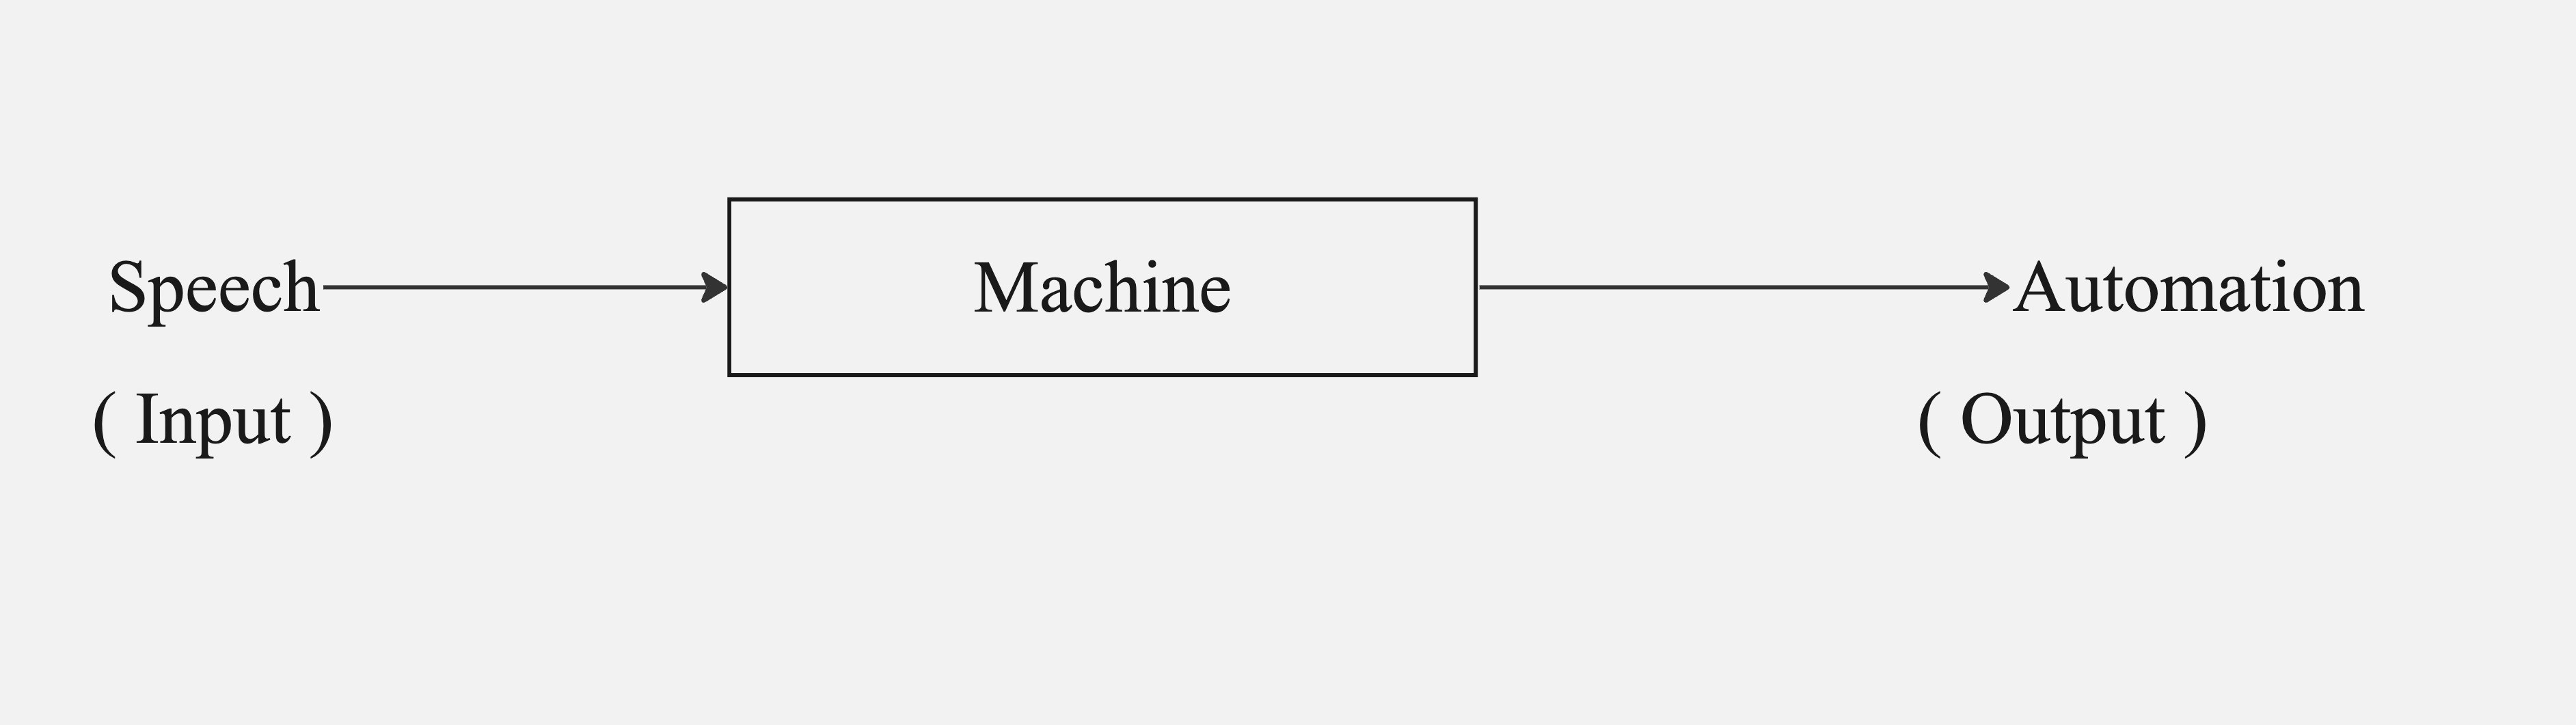
\includegraphics[width=0.9\textwidth]{system1}
            \caption{Block Diagram of Home Automation}
            \label{fig:system1}
        \end{figure}

            Delving deeper into the workings of the system, the process begins with the user providing speech as input through a portable microphone. This input is then transmitted to a Raspberry Pi. Within the Raspberry Pi, a speech-to-text model interprets the spoken words. Upon successful interpretation, the Raspberry Pi generates a signal that commands the control of the appliance(s). This comprehensive system involves multiple components working in tandem to seamlessly translate spoken commands into tangible actions for home automation. The block diagram of the system hardware is shown in \ref{fig:system hardware}.

        \begin{figure}[h]
            \centering
            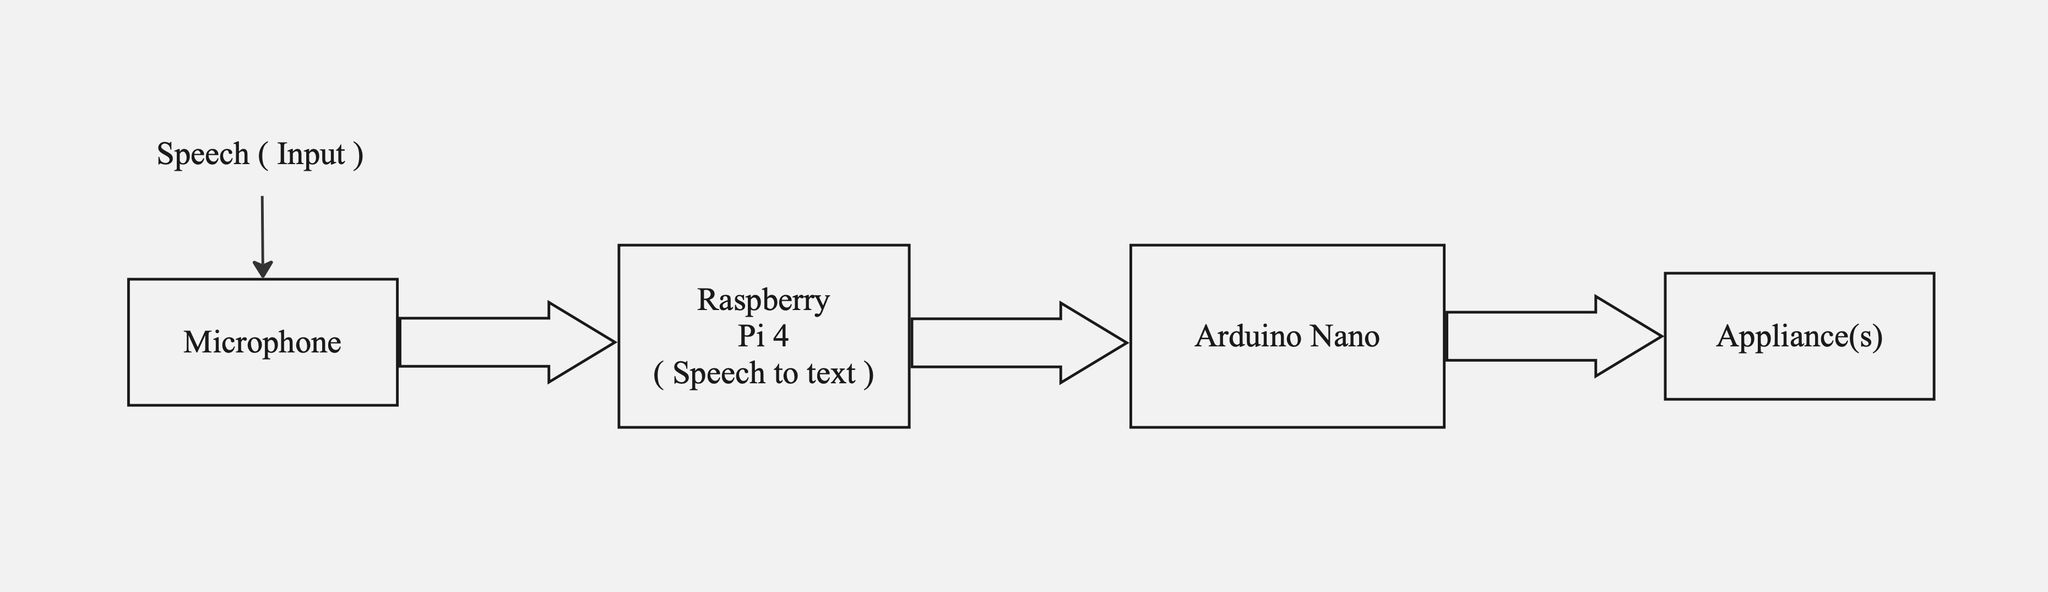
\includegraphics[width=1\textwidth]{system hardware}
            \caption{Block Diagram of System Hardware}
            \label{fig:system hardware}
        \end{figure}

            The process unfolds with the speech serving as input for the speech-to-text model. The converted text undergoes comparison with a wake word in the wake word detector model. If the text does not match a wake word, the system remains inactive until a wake word is detected, prompting the process to restart. Upon recognizing the wake word, the converted text that follows is subjected to a set of conditions, and signals are then dispatched to control the appliances. This iterative sequence ensures that appliance control is contingent on the recognition of a specific wake word, enhancing the system's precision and responsiveness. The flowchart is shown in \ref{fig:system2}.

        \begin{figure}[h]
            \centering
            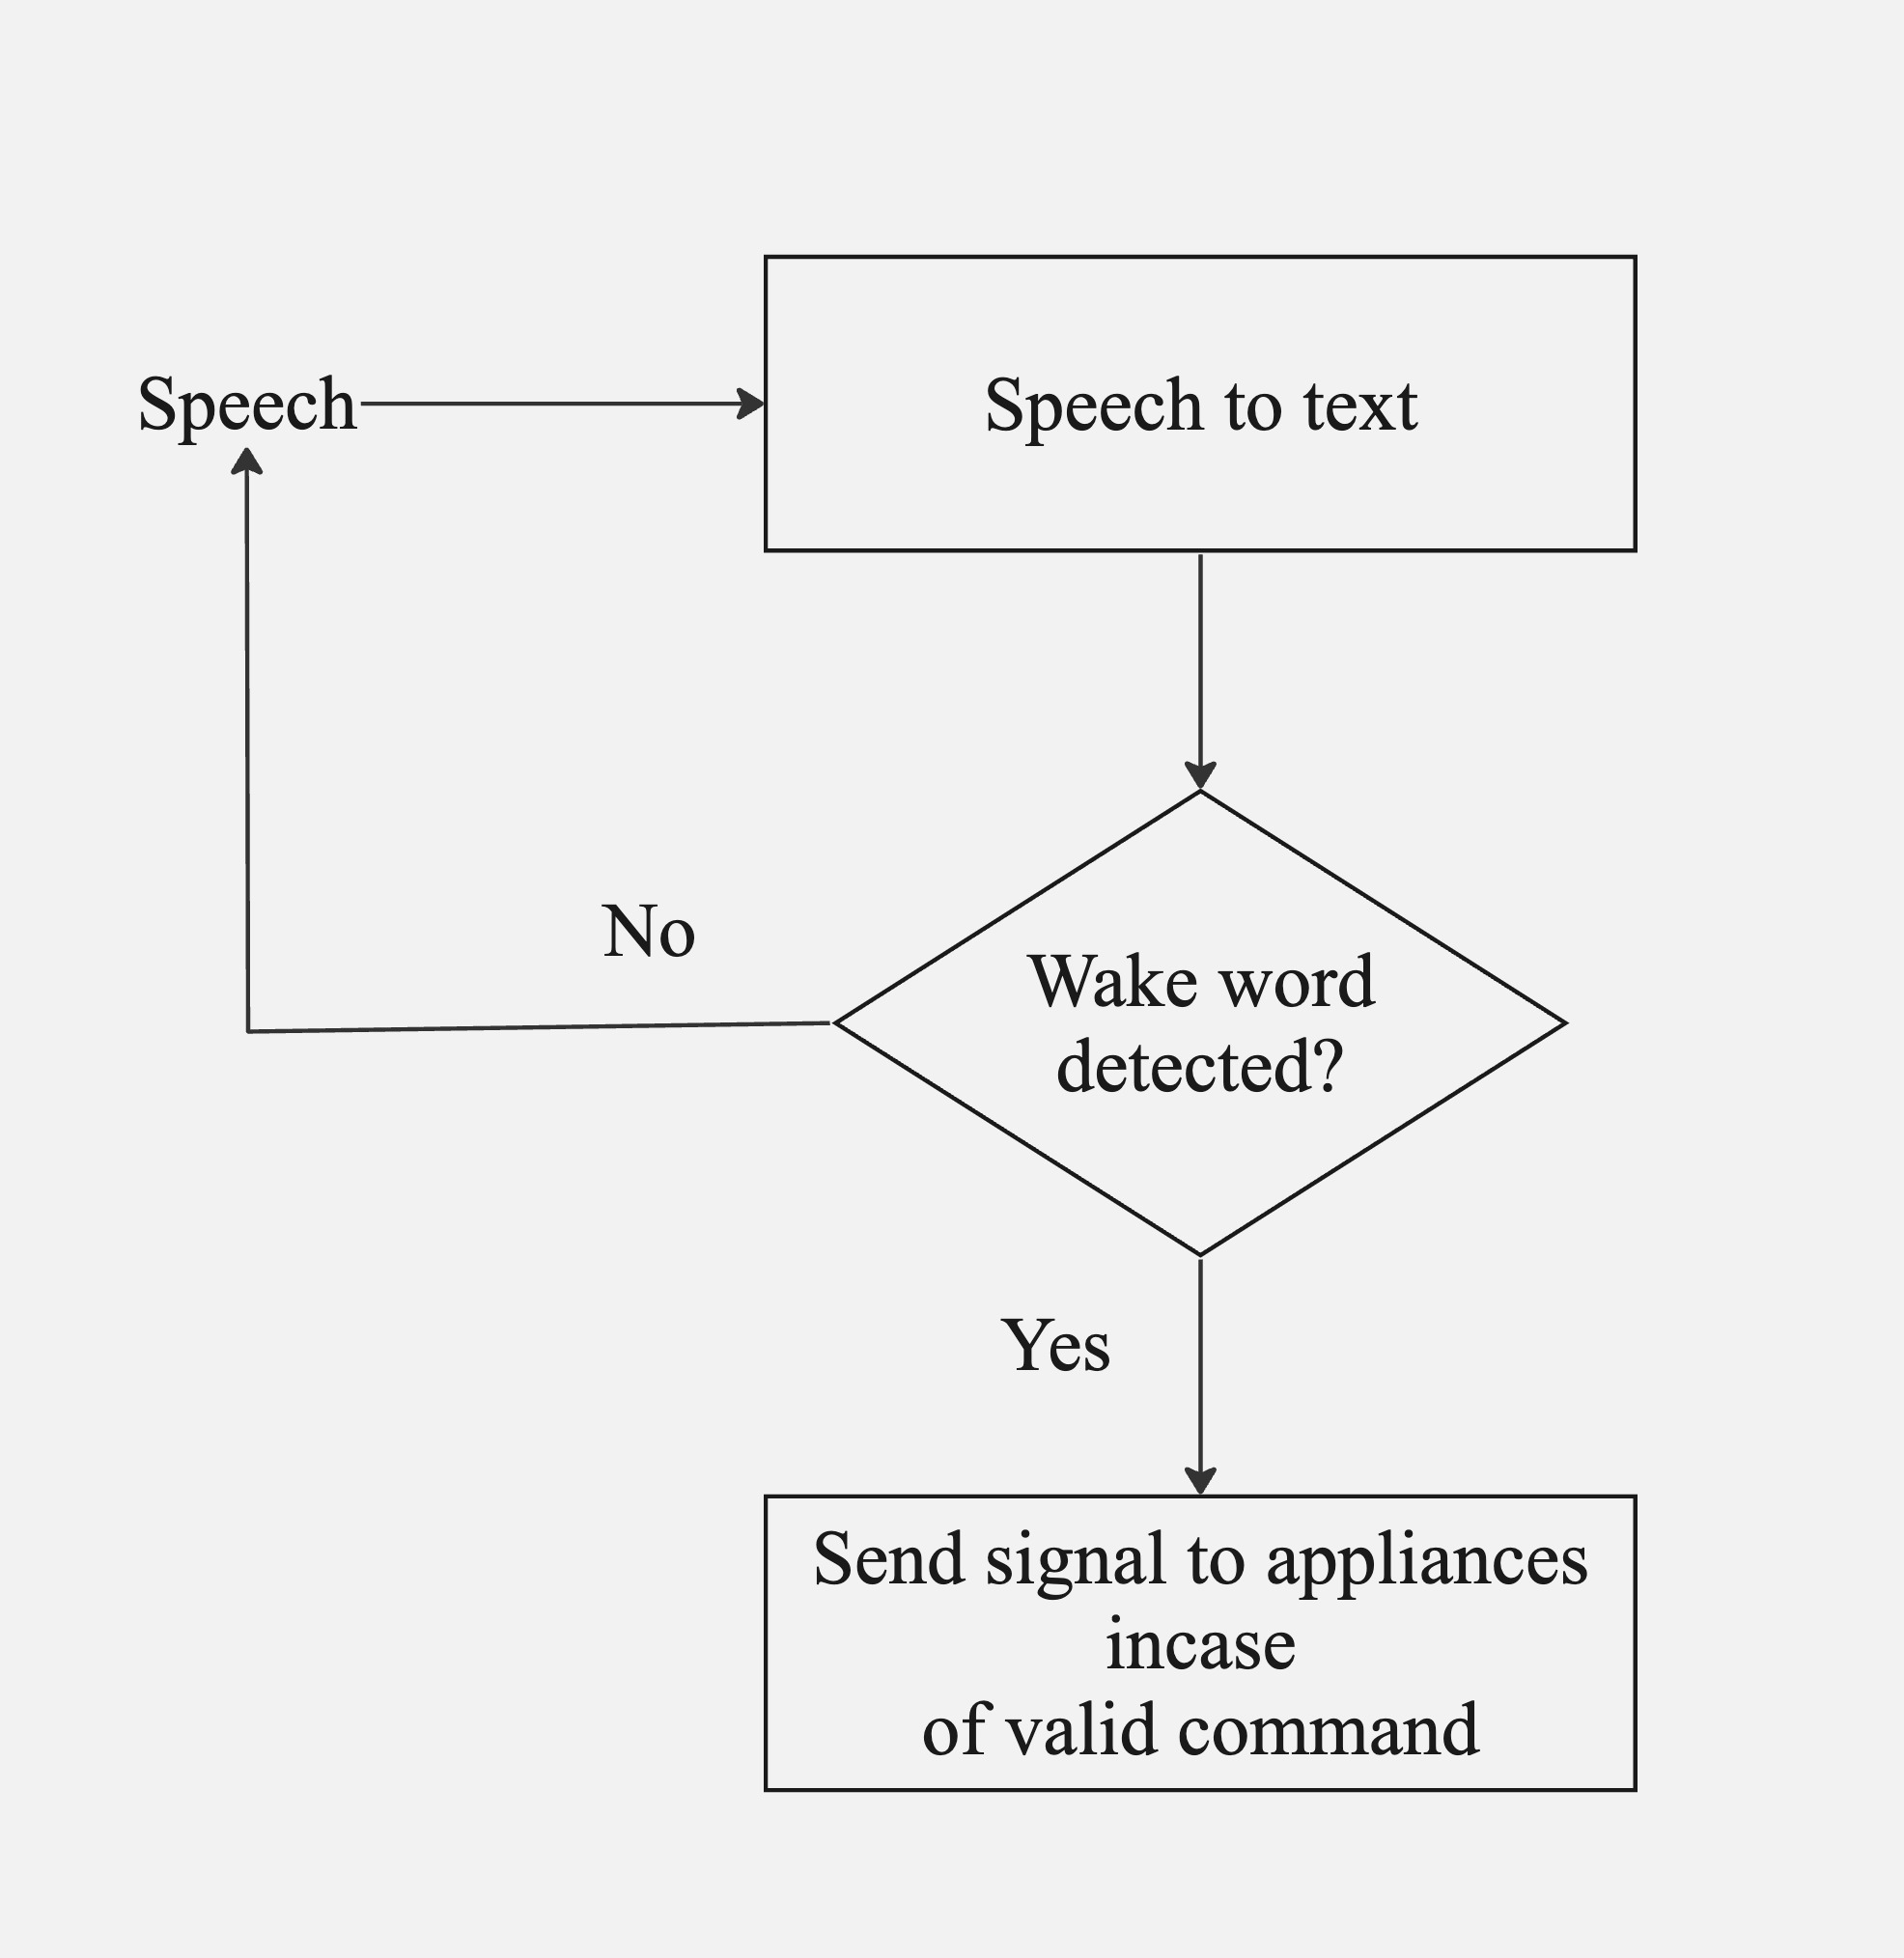
\includegraphics[width=1\textwidth]{system2}
            \caption{Flowchart of Speech Recognition}
            \label{fig:system2}
        \end{figure}
            
       \section{Selection of Raspberry Pi 4 Model B}
       The Raspberry Pi 4 Model B was chosen for our home automation project due to its robust performance, and versatile connectivity. With its quad-core ARM Cortex-A72 processor and adequate memory options, it efficiently executes complex algorithms such as speech recognition. Its built-in Wi-Fi, Bluetooth, USB ports, and GPIO pins facilitate integration with peripheral devices like the Arduino Nano, enabling straightforward hardware control. Overall, the Raspberry Pi 4 Model B serves as the fundamental of our project, offering powerful performance, and reliability to meet the demands of our home automation system.
\newpage
        \section{Activity diagram}
        \begin{figure}[htbp] 
            \centering
            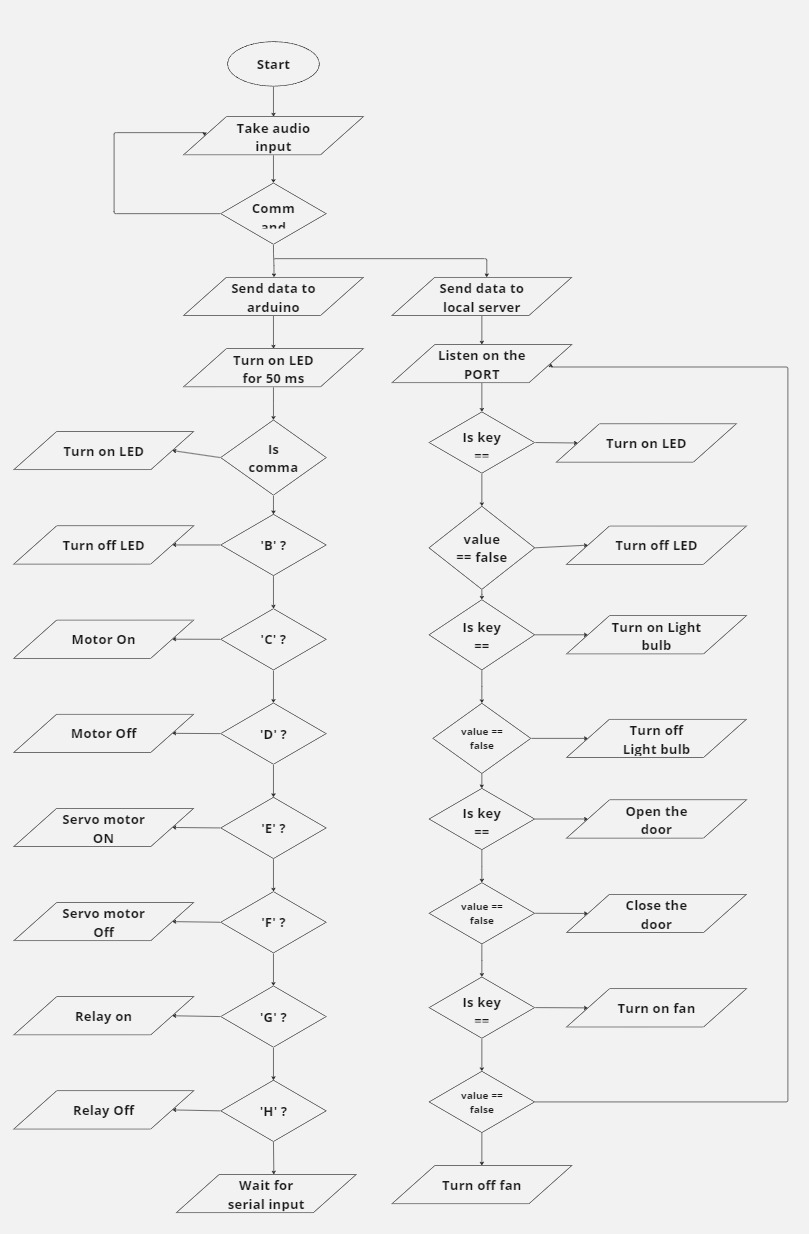
\includegraphics[height=0.7\textheight]{finalact}
            \caption{Activity Diagram}
            \label{fig:Activity}
        \end{figure}
\newpage

        \section{Interfacing between Raspberry Pi 4 Model B and components}
        \begin{figure}[h]
            \centering
            \includegraphics[width=1\textwidth]{interfacing}
            \caption{Interfacing}
            \label{fig:interface}
        \end{figure}
        The Raspberry Pi 4 Model B serves as our development board, which oversees the functions of different hardware elements that, in turn, regulates  the operations of household fixtures. The figure below shows all the interfacing of the home automation system.

        
        From the above diagram, we are illustrating the interfacing between different components present in our system. We are using Raspberry Pi 4 Model B as our development board which uses ARM Cortex-A72 CPU. Control Signal is transmitted from the USB port of the Raspberry Pi to Arduino Nano.The Arduino Nano controls the actions of fixtures. The fixtures are controlled by the signal received from Arduino Nano. External power is provided to the hardware components if needed.\\
        Hence, this is the interfacing between all our components of hardware, i.e Raspberry Pi, Arduino Nano, Relay module, LED, Servo motor, Motor driver and DC motor.

        \section{Interfacing between Hardware and Application}
        The Raspberry pie contains the inbuilt Wi-Fi module which enables the system to come online so a local server is set up. The local server acts as a bridge between the web application and the Raspberry pie. When a command is given to the system then it sends the string to the Arduino Nano via serial communication along with a ‘/post’ request to send the json data for the change in status of the device. Similarly at the website there is a continuous ‘http.get()’ request to fetch the status in realtime, which is then used to change the status of devices in the webpage. Users can see the changes in real time via dashboard.

        \begin{figure}[h]
            \centering
            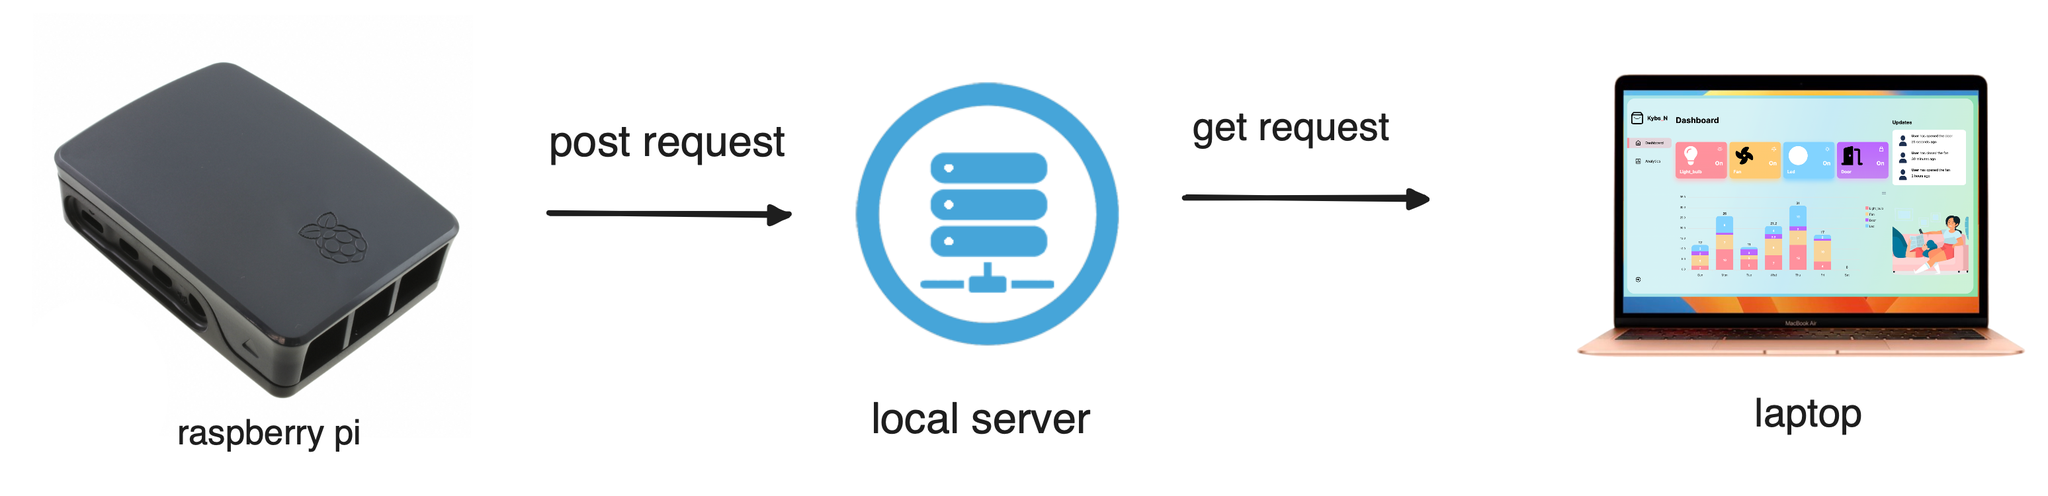
\includegraphics[width=1\textwidth]{hardware_interface}
            \caption{Interfacing between Hardware and Application}
            \label{fig:hardware_interface}
        \end{figure}

        
\chapter{EXPECTED OUTPUT}

\chapter{EPILOGUE}
\section{CONCLUSION}

\section{LIMITATIONS}

\section{FUTURE ENHANCEMENT}


\newpage

\bibliographystyle{unsrt}
\bibliography{refrences/ref.bib}
\addcontentsline{toc}{chapter}{REFERENCES}


\appendix
\chapter{APPENDIX}
Project Timeline
\addcontentsline{toc}{chapter}{ANNEX}
\end{document}

% %%code copied by 
% % %IOE Latex Template originally
% % %prepared by Ramesh Bhandari 072/MSI/610
% % % modified by Dr. Basanta Joshi

% %Page layout setup
% \documentclass[12pt,a4paper,oneside]{report}
% \usepackage[left=1.5in, right=1in,top=1in,bottom=1in,headheight=6pt, a4paper]{geometry}


% %Package imports
% \usepackage{multirow}
% \usepackage{rotating}
% \usepackage{hhline}
% \usepackage{graphicx}
% \graphicspath{{./Graphics/}} 
% \usepackage{titling}
% \usepackage{booktabs}
% \usepackage{natbib}
% \usepackage{microtype}
% \usepackage{amsmath}
% \usepackage{enumitem}
% \usepackage[font=normalsize,labelfont=bf,tableposition=top]{caption}
% \usepackage{setspace}
% \usepackage[explicit]{titlesec}
% \usepackage{tabto}
% \usepackage[hidelinks]{hyperref}
% \usepackage[justification=centering]{caption}


% %Line spacing
% \renewcommand{\baselinestretch}{1.5}
% \setlength{\parskip}{0em}

% %Paragraph indentation
% \setlength{\parindent}{0em}

% %Chapter formatting
% \titleformat{\chapter}[display]
%     {\centering\normalfont\normalsize\bfseries}{\MakeUppercase{\chaptertitlename} \thechapter}{5pt}{\normalsize #1}
% \titlespacing{\chapter}{0pt}{0pt}{20pt}

% %Heading-1 formatting
% \titleformat{\section}
%   {\normalfont\normalsize\bfseries}{\thesection}{1em}{#1}

% %Heading-2 formatting
% \titleformat{\subsection}
%   {\normalfont\normalsize}{\thesubsection}{1em}{#1}

% %Heading-3 formatting
% \titleformat{\subsubsection}
%   {\normalfont\normalsize}{\thesubsubsection}{1em}{#1}

% %Table caption formatting
% \captionsetup[table]{singlelinecheck=off}

% %Metadata
% \title{IMAGE COLORIZATION USING CONVOLUTIONAL NEURAL NETWORK }
% \author{YOUR NAME}
% \date{\today}


% \renewcommand{\bibname}{REFERENCES}
% \renewcommand\contentsname{TABLE OF CONTENTS}
% \renewcommand{\listfigurename}{LIST OF FIGURES}
% \renewcommand{\listtablename}{LIST OF TABLES}


% \begin{document}
    
%     %Include cover page
%     \begin{titlingpage} 
    \begin{normalsize}
    \begin{center}
    
\includegraphics[width=1.3in, height=1.5in]{./Graphics/logo.png}\\
    
     \textbf{TRIBHUVAN UNIVERSITY}\\
     \textbf{INSTITUTE OF ENGINEERING}\\
    
    \textbf{\MakeUppercase PASHCHIMANCHAL CAMPUS}\\
    \textbf{\MakeUppercase{Lamachaur, Pokhara}}
    \end{center}
    \vspace{1cm}
    
    \begin{center}
    \textbf{[Subject Code: EX654]}\\
    \textbf{A PROJECT REPORT}\\
    \textbf{ON}\\
    \textbf{\MakeUppercase \thetitle} \\
    \vspace{1.5 cm}
    \textbf{SUBMITTED BY:}\\
\begin{tabular}{p{5cm} l}
    \textbf{BINAYAK SHRESTHA} & [WRC077BEI012]\\
    \textbf{PRAKANDA BHANDARI} & [WRC077BEI030]\\
    \textbf{PRATHAM ADHIKARI} & [WRC077BEI032]\\
    \textbf{SANDESH BASHYAL} & [WRC077BEI036]\\
\end{tabular}\\
    \vspace{2 cm}
    \textls{\textbf{SUBMITTED TO: }}\\
    \textbf{DEPARTMENT OF ELECTRONICS AND COMPUTER ENGINEERING}\\
    %\MakeUppercase {Pashchimanchal Campus, Lamachaur-16, Pokhara}\par\\
    \vspace{1.5cm}
    \textbf{
    {\monthyeardate\today}}
    \end{center}
    \end{normalsize}
    \end{titlingpage}
    %================================================================
    \newpage
    
%     %Include abstract
%     
\chapter*{ABSTRACT}

\addcontentsline{toc}{chapter}{ABSTRACT}

This section consists of summary of the context

%New Paragraph
\par
\textbf{Keywords:} Deep Learning, Image colorization, EfficientNetB0, CNN, Convolution neural architecture


    
%     %Table of contents
%     \addcontentsline{toc}{chapter}{\contentsname}{\tableofcontents}
    
%     %List of figures
    
%     \newpage
%     \addcontentsline{toc}{chapter}{\listfigurename}{
%         %
%         \let\oldnumberline\numberline%
%         \renewcommand{\numberline}{\figurename~\oldnumberline}%
%         \listoffigures
%         %
%     }
    
%     %List of tables
%     \newpage
%     \addcontentsline{toc}{chapter}{\listtablename}{
%         %
%         \let\oldnumberline\numberline%
%         \renewcommand{\numberline}{\tableautorefname~\oldnumberline}%
%         \listoftables
%         %
%     }
    
%     \newpage
%     \chapter*{LIST OF ABBREVIATIONS}
\addcontentsline{toc}{chapter}{LIST OF ABBREVIATIONS}
%Add abbreviations list here
AI\tabto{6em}Artificial Intelligence\\
CNN\tabto{6em} Convolution Neural Network\\
%     \pagenumbering{arabic}
\setcounter{page}{1}
\chapter{INTRODUCTION}
    \section{Background}
    In the contemporary era of smart living, home automation systems have become increasingly popular due to their ability to enhance convenience, efficiency and also catering to individuals with mobility challenges. Integration of speech recognition technology into home automation systems adds an additional layer of user-friendliness, accessibility, leveraging its power to seamlessly interact with various devices within a home environment.

    Traditional method with physical switching of appliances, checking if they are on or not brings a level of inconvenience to disabled as well as abled people. This system can accurately interpret the user instructions and generates control signals for appliances. It does so by capturing audio input through a connected microphone.

    Upon receiving the audio signals, Raspberry pi utilizes a speech recognition model within it which converts the received voice data into text commands enabling the system to comprehend user instructions accurately. Once the command is interpreted, It then generates necessary control signals and sends them to a 1-channel relay module and other hardware components, allowing a seamless control of different household appliances connected to the system. The status of the appliances are updated in real-time which can be viewed on a dashboard of a web application. This system not only operates the appliances, but also views their status which makes it easier to observe them  even if  not physically present near them.

    \section{Motivation and Inspiration}
    Our project's motivation and inspiration stemmed from a genuine desire to simplify and improve daily life within homes. Witnessing the growing integration of technology into our lives, we were inspired to utilize advancements in speech recognition and automation to make household tasks more efficient and accessible. Our goal was to empower users with intuitive control over their environment, aiming for a user-friendly home automation system. Additionally, we were excited about the opportunity to explore the intersection of artificial intelligence, embedded systems, and IoT technologies, seeing it as a chance to deepen our understanding and expertise in these areas. 
    
    \section{Problem Statement}
    The absence of automated controls requires manual operation of various appliances and thus results in a time consuming routine. Managing multiple devices  manually  can be troublesome especially for elderly and the disabled. The commercial home automation systems are based mainly on Zigbee, Z-Wave, or Wi-Fi protocols. Such automated systems are either ineffective in terms of cost or power consumption. 

    Additionally, the complexity of processing speech in real-time poses a significant challenge. Existing systems often struggle with accurately interpreting the intent of the speaker. Thus, the technologies that are being applied are prone to various kinds of failures, for instance an individual’s speech can be misinterpreted,in case of multiple commands by more than one person the commands might be neglected. 

    
    \section{Objectives}
    The objectives of this project is:
        \begin{itemize}
        %define spacing
        \setlength\itemsep{1.5pt}
        %Add items
        \item To design and develop a speech recognizing home automation system that can comprehend user instructions accurately and operates accordingly.

        \end{itemize}


    \section{Scope}
    Our project's scope involves creating a comprehensive home automation system that merges speech recognition technology with hardware automation to improve household functionality. Our main goal is to develop an easy-to-use interface enabling residents to control various home fixtures and devices through voice commands. 

    We also plan to incorporate features for task scheduling, such as setting timers and activating predefined routines, to streamline daily routines further. The Raspberry Pi 4 Model B will serve as the central controlling unit, facilitating communication between the speech recognition algorithm and connected hardware components through the Arduino Nano. While our initial focus is on essential features, we're designing the system to be scalable, allowing for future expansions and updates to meet changing user needs and technological advancements in home automation.
         
%     \chapter{LITERATURE REVIEW}

Recurrent neural networks, long short-term memory and gated recurrent neural networks in particular, was firmly established as state of the art approaches in sequence modeling and transduction problems such as language modeling and machine translation. Numerous efforts have since continued to push the boundaries of recurrent language models and encoder-decoder architectures \cite{vaswani2017attention}.Recurrent Neural Networks (RNNs) and their variant LSTMs, while powerful, suffer from limitations. LSTMs attempt to address the vanishing gradient problem in RNNs, where crucial information from earlier parts of the sequence gets lost. However, LSTMs can still struggle with very long sequences. Additionally, both RNNs and LSTMs process information sequentially, limiting their ability to capture complex relationships within the data. This sequential nature also makes them computationally expensive for training. These drawbacks hinder their performance in tasks requiring long-range dependencies and efficient processing, paving the way for advancements like transformers.
\newline The drawbacks of these models being inability to generalize to long sequences, unparalizability are solved by Transformer.Transformers\cite{vaswani2017attention} outperform LSTMs in sequence modeling tasks like machine translation due to their powerful attention mechanism. Unlike LSTMs, which process information sequentially, transformers can attend to all parts of the input sequence simultaneously using self-attention. This allows them to capture long-range dependencies more effectively, crucial for understanding complex relationships in language. Additionally, encoders and decoders within transformers are specifically designed to handle input and output sequences, respectively, leading to better focus and efficiency compared to LSTMs' single, recurrent processing. This combination of self-attention and dedicated encoder-decoder architecture grants transformers superior accuracy in various NLP tasks. \\

For Automatic speech recognition, new speech recognition model using attention-based recurrent networks was used \cite{effectivenesschorowski2015attention}. Unlike traditional methods, the model can focus on important parts of the speech throughout the sequence. This is useful for long and noisy speech recognition tasks. The model was tested  on a phoneme recognition task and show that it performs competitively, especially for longer speech samples.\cite{effectivenesschorowski2015attention}. \newline

The Transformer model was first introduced in Gaussian mixture hidden Markov modeling for speech recognition\cite{1198704}, in order to reduce sequential calculations and the number of operations for correlating input and output position signals\cite{orken2022study}.The model performed exceptionally well in compared to state-of-the-art models at the time.

Speech recognition relies on labeled data, limiting its reach. Baevski \cite{baevski2021unsupervised} proposes wav2vec-U, an unsupervised method using self-supervised learning from wav2vec 2.0 representations. k-means clustering segments speech, and adversarial training maps segments to phonemes, even allowing for silence labels. wav2vec-U achieves significant reductions in phone error rates on TIMIT and rivals supervised models on Librispeech, demonstrating its effectiveness across languages. This approach paves the way for speech recognition in low-resource settings. Experiments on the standard Librispeech benchmark show performance close to the state of the art models from only a few years ago, even though these models relied on nearly 1,000 hours of labeled data\cite{baevski2021unsupervised}. \newline

The model, Whisper, leverages a massive dataset of audio recordings with corresponding, but imperfect, internet transcripts. This weak supervision approach, alongside multilingual and multitask training, allows Whisper to excel in zero-shot generalization and achieve competitive performance compared to fully supervised models. Furthermore, Whisper simplifies the recognition pipeline by eliminating the text normalization step. These findings highlight the potential of weak supervision for robust and efficient speech recognition.The smallest zero-shot Whisper model, which has only 39 million parameters and a 6.7 WER on LibriSpeech test-clean is roughly competitive with the best supervised LibriSpeech model when evaluated on other datasets \cite{whisper}.Whisper showed high transcription performances (for each language the percentage of correct words transcribed is higher than 90\%). For the English and Italian languages, the most committed mistakes were words substitutions, while for Russian there were observed higher percentages of both words substitution and insertion errors \cite{amorese2023automatic}. \newline
%     \chapter{RELATED THEORY}
\section{Section1}
        \subsection{Subsection}
        \begin{enumerate}[label=\alph*.]
            \item Sub subsection
        
          \begin{figure}[ht]
            \centering
            \includegraphics[width=0.55\textwidth]{Graphics/Outline-of-the-convolutional-layer_W640.jpg}\\
            \caption{Basic Outline of a Convolutional Layer}
        \end{figure}\\
        
Where,
        %Equation example
        \begin{equation}
            C(X, \theta)=\frac{1}{2HW}\sum_{k\in{a,b}}\sum_{i=1}^{H} \sum_{j=1}^{W} (Xk_i,_j - \overset{\sim}{X}k_i,_j)^2
             \end{equation}
         
        where $\theta$ represents all model parameters,$Xk_i,_j$ and denote the ij:th pixel value of the k:th component of the target and reconstructed image, respectively. This can easily be extended to be a batch $\beta$ by averaging the cost among all images in the batch, i.e. $1/|\beta|\sum_{X\in_{\beta}} C(X,\theta)$.\\
        \end{enumerate}
%     \include{section/methodlogy}
%     \include{section/expected_output}
%     \newpage
    
%     \bibliographystyle{unsrt}
%     \bibliography{refrences/ref.bib}
%     \addcontentsline{toc}{chapter}{REFERENCES}
%     \appendix
\chapter{APPENDIX}
Project Timeline

% \end{document}

